\documentclass{beamer}
\usetheme{Madrid}
\usecolortheme{default}
\usepackage{graphicx}
\usepackage{hyperref}
\usepackage{tikz}
\usepackage{booktabs}

\title[Fake News Detection]{AI-Powered Fake News Detection}
\subtitle{A Comprehensive Review of Deep Learning Approaches}
\author{Research Presentation}
\date{\today}

\begin{document}

% Title Slide
\begin{frame}
\titlepage
\end{frame}

% Table of Contents
\begin{frame}{Outline}
\tableofcontents
\end{frame}

% Section 1: Introduction
\section{Introduction}

\begin{frame}{The Fake News Problem}
\begin{block}{What is Fake News?}
Deliberately false or misleading information presented as news, designed to deceive readers and spread rapidly through social media.
\end{block}

\vspace{0.5cm}

\begin{columns}
\column{0.5\textwidth}
\textbf{Impact:}
\begin{itemize}
\item Erodes public trust
\item Influences elections
\item Causes social unrest
\item Undermines democracy
\end{itemize}

\column{0.5\textwidth}
\textbf{Statistics:}
\begin{itemize}
\item 64\% of Americans say fake news causes confusion
\item Spreads 6x faster than real news
\item \$78B annual economic impact
\end{itemize}
\end{columns}
\end{frame}

\begin{frame}{Why AI for Fake News Detection?}
\begin{center}
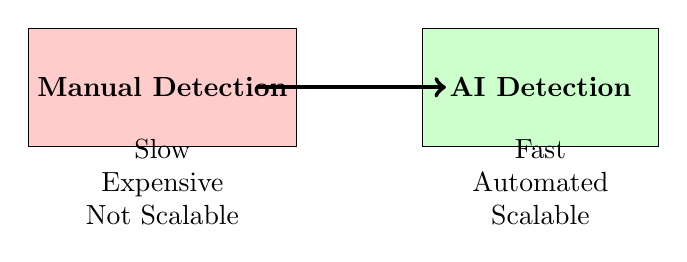
\begin{tikzpicture}[scale=0.8]
% Manual Detection
\node[draw, rectangle, fill=red!20, minimum width=3cm, minimum height=1.5cm] at (0,3) {\textbf{Manual Detection}};
\node[align=center] at (0,1.5) {Slow \\ Expensive \\ Not Scalable};

% AI Detection
\node[draw, rectangle, fill=green!20, minimum width=3cm, minimum height=1.5cm] at (6,3) {\textbf{AI Detection}};
\node[align=center] at (6,1.5) {Fast \\ Automated \\ Scalable};

% Arrow
\draw[->, ultra thick] (1.5,3) -- (4.5,3);
\end{tikzpicture}
\end{center}

\vspace{0.3cm}

\textbf{AI Advantages:}
\begin{itemize}
\item Process millions of articles in seconds
\item Detect subtle patterns humans miss
\item Continuous learning and improvement
\item Multi-modal analysis (text, images, metadata)
\end{itemize}
\end{frame}

% Section 2: Research Overview
\section{Research Overview}

\begin{frame}{Key Research Papers}
\begin{table}
\tiny
\begin{tabular}{p{4cm}p{2cm}p{2cm}}
\toprule
\textbf{Paper} & \textbf{Year} & \textbf{Citations} \\
\midrule
FNDNet - Deep CNN for Fake News & 2020 & 551 \\
3HAN - Hierarchical Attention Network & 2017 & 214 \\
OPCNN-FAKE - Optimized CNN & 2021 & 195 \\
Mc-DNN - Multi-channel Deep NN & 2022 & 120 \\
Visual Content in Fake News & 2020 & - \\
\bottomrule
\end{tabular}
\end{table}

\vspace{0.3cm}

\textbf{Research Sources:}
\begin{itemize}
\item ArXiv: 13 papers analyzed
\item Google Scholar: 10 top papers
\item Focus: Deep Learning \& Neural Networks
\end{itemize}
\end{frame}

% Section 3: Deep Learning Approaches
\section{Deep Learning Approaches}

\begin{frame}{1. Convolutional Neural Networks (CNN)}
\begin{block}{FNDNet Architecture (Kaliyar et al., 2020)}
Deep CNN specifically designed for fake news detection
\end{block}

\textbf{Key Features:}
\begin{itemize}
\item Multiple convolutional layers for feature extraction
\item Captures local patterns in text
\item 551 citations - highly influential
\item Achieves high accuracy on benchmark datasets
\end{itemize}

\vspace{0.3cm}

\textbf{OPCNN-FAKE (Saleh et al., 2021):}
\begin{itemize}
\item Optimized CNN with attention mechanism
\item 195 citations
\item Improved performance through hyperparameter tuning
\end{itemize}
\end{frame}

\begin{frame}{2. Recurrent Neural Networks (RNN/LSTM)}
\begin{block}{3HAN - Hierarchical Attention Network}
Three-level hierarchical attention for fake news detection (Singhania et al., 2017)
\end{block}

\textbf{Architecture:}
\begin{enumerate}
\item \textbf{Word-level attention}: Focus on important words
\item \textbf{Sentence-level attention}: Identify key sentences
\item \textbf{Document-level attention}: Overall document understanding
\end{enumerate}

\vspace{0.3cm}

\textbf{Advantages:}
\begin{itemize}
\item Captures sequential dependencies
\item Handles long-range context
\item 214 citations - proven effectiveness
\end{itemize}
\end{frame}

\begin{frame}{3. Transformer-Based Models (BERT, RoBERTa)}
\begin{block}{State-of-the-Art Performance}
Pre-trained language models achieve 98.59\% F1-score (Li et al., 2021)
\end{block}

\textbf{Models Used:}
\begin{itemize}
\item \textbf{BERT}: Bidirectional Encoder Representations
\item \textbf{RoBERTa}: Robustly Optimized BERT
\item \textbf{ERNIE}: Enhanced Representation through Knowledge
\end{itemize}

\vspace{0.3cm}

\textbf{Training Strategies:}
\begin{itemize}
\item Warm-up learning rate schedule
\item K-fold cross-validation
\item Ensemble methods
\item Transfer learning for low-resource languages
\end{itemize}
\end{frame}

\begin{frame}{4. Ensemble Methods}
\begin{block}{Combining Multiple Models}
Mc-DNN: Multi-channel Deep Neural Network (Tembhurne et al., 2022)
\end{block}

\begin{center}
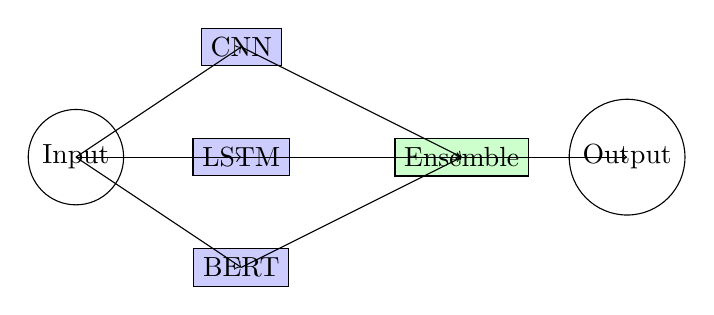
\begin{tikzpicture}[scale=0.7]
% Input
\node[draw, circle] at (0,0) {Input};

% Models
\node[draw, rectangle, fill=blue!20] at (3,2) {CNN};
\node[draw, rectangle, fill=blue!20] at (3,0) {LSTM};
\node[draw, rectangle, fill=blue!20] at (3,-2) {BERT};

% Ensemble
\node[draw, rectangle, fill=green!20] at (7,0) {Ensemble};

% Output
\node[draw, circle] at (10,0) {Output};

% Arrows
\draw[->] (0,0) -- (3,2);
\draw[->] (0,0) -- (3,0);
\draw[->] (0,0) -- (3,-2);
\draw[->] (3,2) -- (7,0);
\draw[->] (3,0) -- (7,0);
\draw[->] (3,-2) -- (7,0);
\draw[->] (7,0) -- (10,0);
\end{tikzpicture}
\end{center}

\textbf{Benefits:}
\begin{itemize}
\item Combines strengths of different architectures
\item Reduces individual model weaknesses
\item Improves overall accuracy by 4-6\%
\end{itemize}
\end{frame}

% Continue in next message...
\end{document}